\begin{document}
	\chapter{Results}
	
	The study conducted over the gathered data served for the definition of new metrics to measure the performance and robustness of the Lightning Network and for the formal modeling of two mathematical representation of the Lightning Network, from a static and dynamic point of view. The analysis is carried over a period of one month, one snapshot per day; this observation period will be justified by the results obtained by the analysis of daily behavior of the network that will be shown next.
	
	\section{Trends}
	
	The following section takes in consideration the most relevant trends of the network which are the nodes and edges variation, the average degree and the diameter of the network on a daily and a monthly basis. The analysis carried over the daily basis data is made to justify the decision of the focus on a larger time window. The reasons behind the following churn rates are out of the scope of this work, but it is likely that they largely depends on protocol changes, client errors and, possibly the popularity of the network itself.
	
	A full day representation of the Lightning Network consists of 144 snapshots taken at 10 minutes intervals; the 10 minutes intervals were chosen because every channel that is added (or removed) from the network must wait for the funding transaction (settlement transaction in case a channel is being closed) to be included in a block and added to the chain by the miners. The following results matched the expectation because, as stated in the white paper, a Lightning node and its channels are meant to have a long lifespan. The data refers to the date of 16th of May, 21th of May ,26th of May, 2nd of June, 
	
	\subsection{Daily nodes variation}
	
	\begin{figure}[h]
		\centering
		\begin{subfigure}{0.45\textwidth}
			\centering
			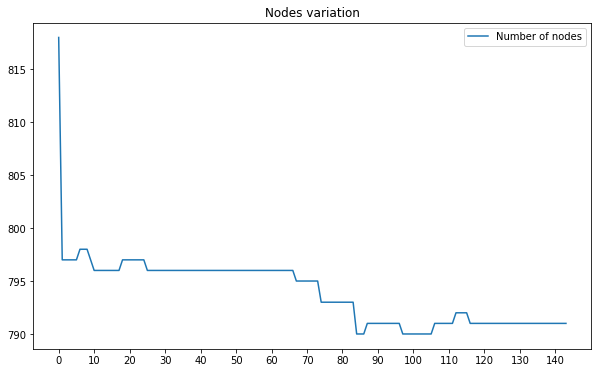
\includegraphics[width=\linewidth]{daily_number_of_nodes0}
			\caption{Snapshot, May 16th}
			\label{daily_node0}
		\end{subfigure}
		\begin{subfigure}{0.45\textwidth}
			\centering
			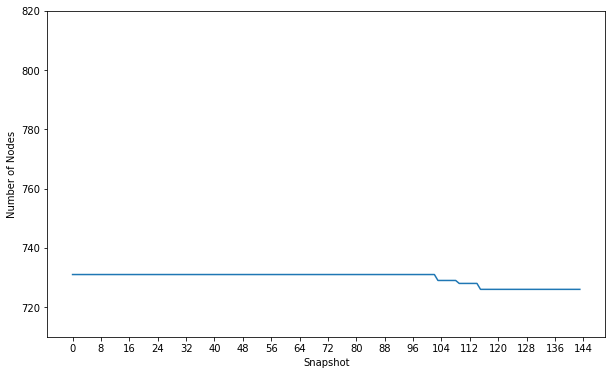
\includegraphics[width=\linewidth]{daily_number_of_nodes1}
			\caption{Snapshot, May 21th}
			\label{daily_node1}
		\end{subfigure}
			\begin{subfigure}{0.45\textwidth}
			\centering
			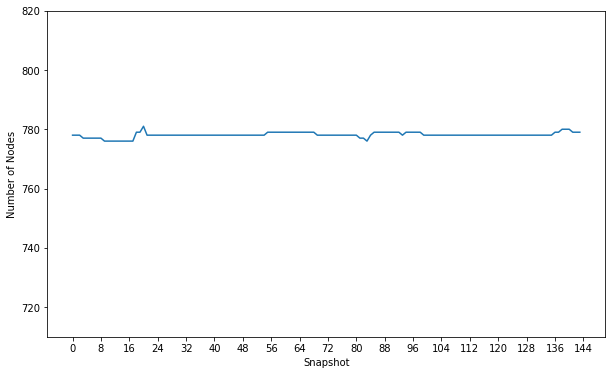
\includegraphics[width=\linewidth]{daily_number_of_nodes2}
			\caption{Snapshot, May 26th}
			\label{daily_node2}
		\end{subfigure}
		\begin{subfigure}{0.45\textwidth}
			\centering
			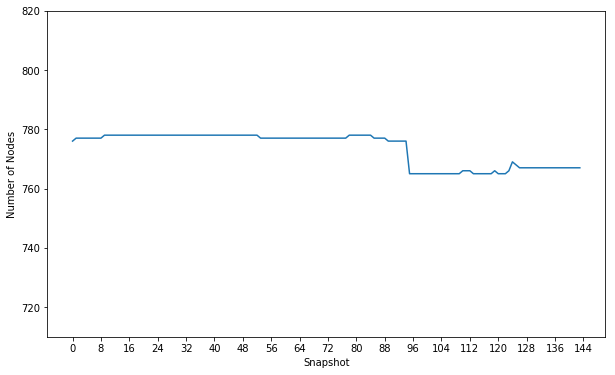
\includegraphics[width=\linewidth]{daily_number_of_nodes3}
			\caption{Snapshot, June 2nd}
			\label{daily_node3}
		\end{subfigure}
		
		\caption{Nodes trends on a daily basis}
		\label{daily_nodes_variation}
	\end{figure}

	Details on nodes variations on a daily basis are reported in \ref{daily_nodes_variation}. The figure shows the 144 snapshot of the network for four different days. We can notice a similar behavior between the snapshots pictured in (\ref{daily_node1}) and (\ref{daily_node3}), although we can't appreciate the same behavior in (\ref{daily_node0}) or (\ref{daily_node2}). 
	
	While the plots may present steep slopes, it has to be noticed that the number of nodes that are joining or leaving the network is actually very low. To figure out better the numbers, the following table will show the percentage variation with respect to the initial state of the network and the highest and lowest order the graph reached that day.
	
	\begin{center}
		\begin{tabulary}{\linewidth}{| L | C | C | C | C |}
			\hline
			 & May 16th (\ref{daily_node0}) & May 21th (\ref{daily_node1}) & May 26th (\ref{daily_node0}) & June 2nd (\ref{daily_node3}) \\
			\hline
			Starting nodes & 818 & 731 & 778 & 776 \\ \hline
			Final nodes & 791 & 726 & 779 & 767 \\ \hline
			Variation(\%) & -3.30\% & -0.68\% & +0.12\% & -1.15\% \\ \hline
			Max number of nodes & 818 & 731 & 781 & 778 \\ \hline
			Min number of nodes & 790 & 726 & 776 & 765 \\ \hline

		\end{tabulary}
	\end{center}
	
	\subsection{Daily edges variation}

	\begin{figure}[h]
		\centering
		\begin{subfigure}{0.45\textwidth}
			\centering
			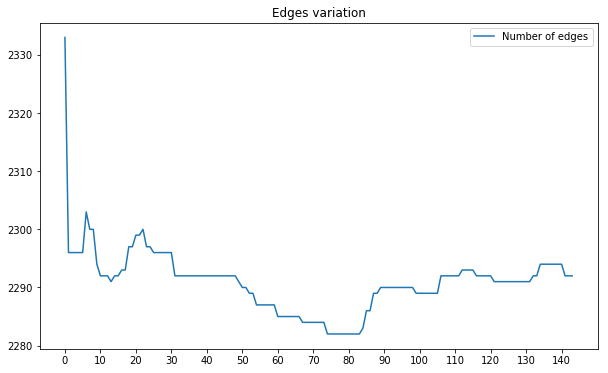
\includegraphics[width=\linewidth]{daily_number_of_edges0}
			\caption{Snapshot, May 16th}
			\label{daily_edges0}
		\end{subfigure}
		\begin{subfigure}{0.45\textwidth}
			\centering
			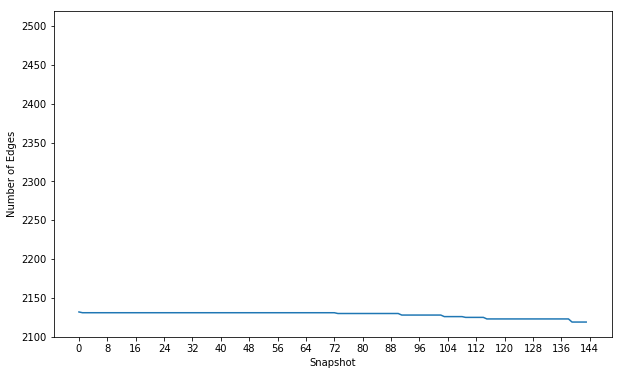
\includegraphics[width=\linewidth]{daily_number_of_edges1}
			\caption{Snapshot, May 21th}
			\label{daily_edges1}
		\end{subfigure}
		\begin{subfigure}{0.45\textwidth}
			\centering
			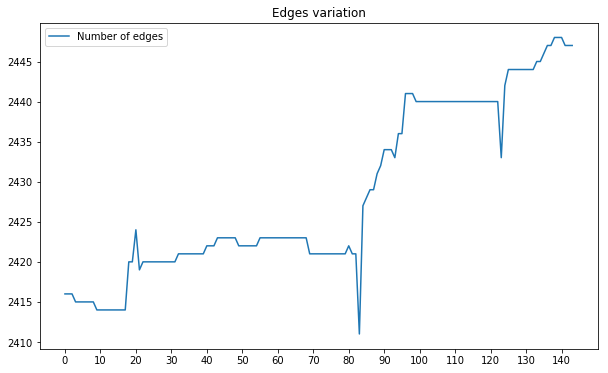
\includegraphics[width=\linewidth]{daily_number_of_edges2}
			\caption{Snapshot, May 26th}
			\label{daily_edges2}
		\end{subfigure}
		\begin{subfigure}{0.45\textwidth}
			\centering
			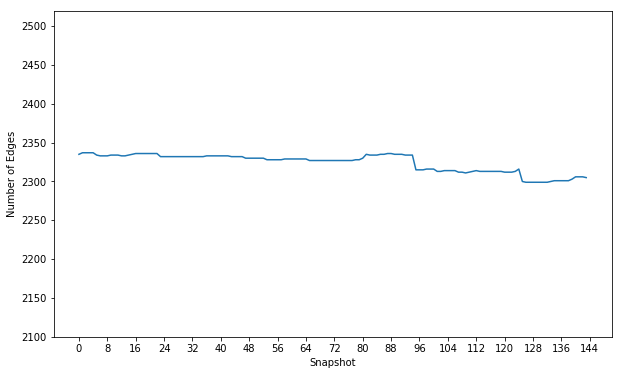
\includegraphics[width=\linewidth]{daily_number_of_edges3}
			\caption{Snapshot, June 2nd}
			\label{daily_edges3}
		\end{subfigure}
		
		\caption{Edges trends on a daily basis}
		\label{daily_edges_variation}
	\end{figure}

	The trends for edges essentially follow the same behavior of the nodes. It is trivial to see that for each node connecting (disconnecting) to the network, at least one channel is added (removed). The actual number of edges per node will be shown in the next section.
	
	\begin{center}
	\begin{tabulary}{\linewidth}{| L | C | C | C | C |}
		\hline
		& May 16th (\ref{daily_edges0}) & May 21th (\ref{daily_edges1}) & May 26th (\ref{daily_edges0}) & June 2nd (\ref{daily_edges3}) \\
		\hline
		Starting edges & 2333 & 2132 & 2416 & 2335 \\ \hline
		Final edges & 2292 & 2119 & 2447 & 2305 \\ \hline
		Variation(\%) & -1.75\% & -0.60\% & +1.28\% & -1.28\% \\ \hline
		Max num. edges & 2333 & 2132 & 2448 & 2337 \\ \hline
		Min num. edges & 2282 & 2119 & 2411 & 2299 \\ \hline	
	\end{tabulary}
	\end{center}

	\subsection{Daily average degree variation}

	\begin{figure}[h]
	\centering
		\begin{subfigure}{0.45\textwidth}
			\centering
			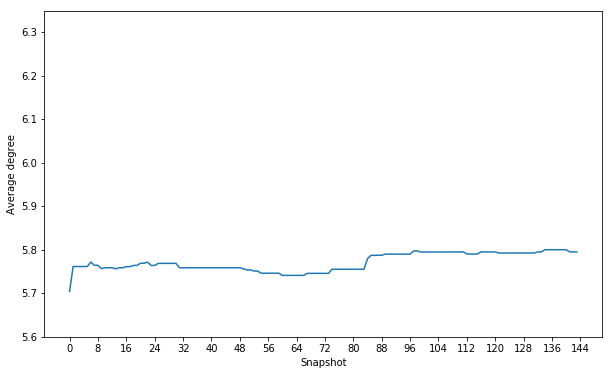
\includegraphics[width=\linewidth]{daily_average_degree0}
			\caption{Snapshot, May 16th}
			\label{daily_degree0}
		\end{subfigure}
		\begin{subfigure}{0.45\textwidth}
			\centering
			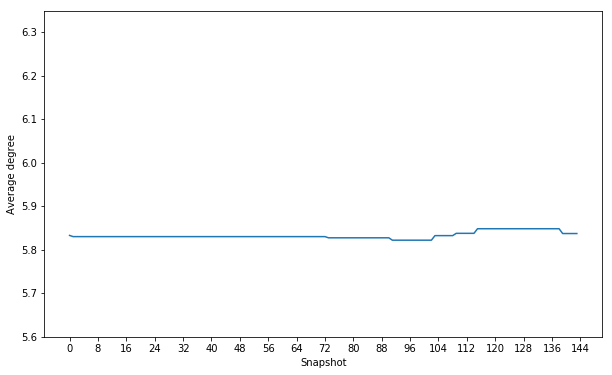
\includegraphics[width=\linewidth]{daily_average_degree1}
			\caption{Snapshot, May 21th}
			\label{daily_degree1}
		\end{subfigure}
		\begin{subfigure}{0.45\textwidth}
			\centering
			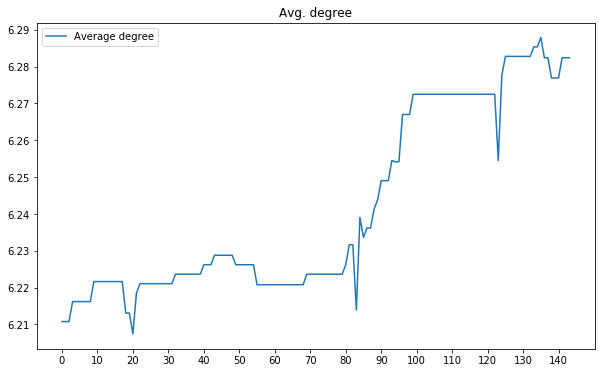
\includegraphics[width=\linewidth]{daily_average_degree2}
			\caption{Snapshot, May 26th}
			\label{daily_degree2}
		\end{subfigure}
		\begin{subfigure}{0.45\textwidth}
			\centering
			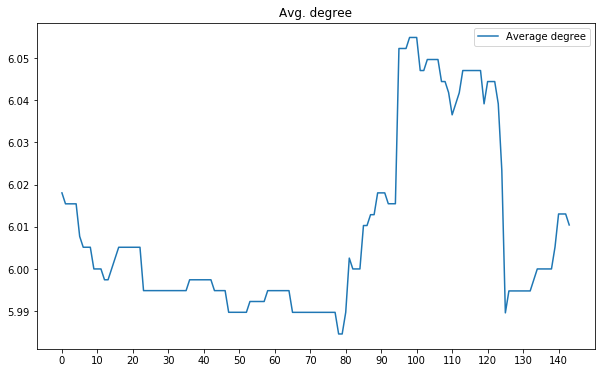
\includegraphics[width=\linewidth]{daily_average_degree3}
			\caption{Snapshot, June 2nd}
			\label{daily_degree3}
		\end{subfigure}
	
	\caption{Average degree on a daily basis}
	\label{daily_degree _variation}
	\end{figure}

	The daily average degree score appears to be confined between an all time highest of 1.59\% and -0.12\% among the days in exam and it is coherent with the number of nodes and edges fluctuation. By putting in relation the number of nodes and average degree variation it is possible to learn more about what kind of nodes are joining or leaving the network: for example data from (\ref{daily_node0}) and (\ref{daily_edges0}) show a negative edges and nodes fluctuation while the average degree variation of (\ref{daily_degree0}) is overall increased, suggesting that the nodes that left the network were actually single-channels node.


	\begin{center}
		\begin{tabulary}{\linewidth}{| L | C | C | C | C |}
			\hline	
			& May 16th (\ref{daily_degree0}) & May 21th (\ref{daily_degree1}) & May 26th (\ref{daily_degree2}) & June 2nd (\ref{daily_degree3}) \\
			\hline
			Starting degree & 5.70 & 5.833 & 6.21  & 6.018 \\ \hline
			Final degree & 5.79 & 5.837 & 6.28 & 6.010 \\ \hline
			Variation (\%) & +1.59\% & +0.07\% & +1.15\% & -0.12\% \\ \hline
			Max avg. degree & 5.80 & 5.84 & 6.28 & 6.05 \\ \hline
			Min avg. degree & 5.70 & 5.82 & 6.20 & 5.98 \\ \hline		
		\end{tabulary}
	\end{center}
	
	\subsection{Daily diameter}
	
		\begin{figure}[h]
		\centering
		\begin{subfigure}{0.45\textwidth}
			\centering
			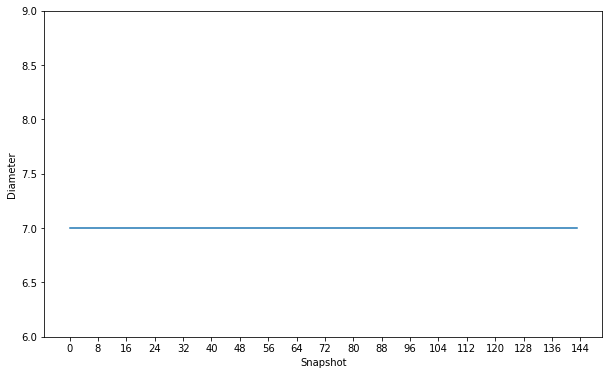
\includegraphics[width=\linewidth]{daily_diameter0}
			\caption{Snapshot, May 16th}
			\label{daily_diameter0}
		\end{subfigure}
		\begin{subfigure}{0.45\textwidth}
			\centering
			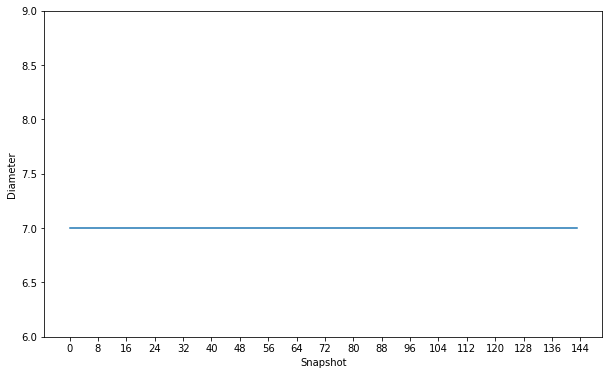
\includegraphics[width=\linewidth]{daily_diameter1}
			\caption{Snapshot, May 21th}
			\label{daily_diameter1}
		\end{subfigure}
		\begin{subfigure}{0.45\textwidth}
			\centering
			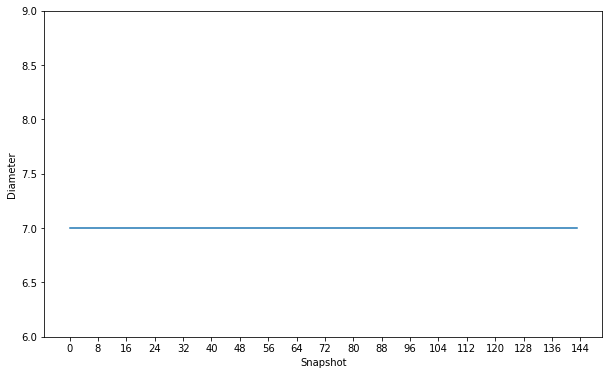
\includegraphics[width=\linewidth]{daily_diameter2}
			\caption{Snapshot, May 26th}
			\label{daily_diameter2}
		\end{subfigure}
		\begin{subfigure}{0.45\textwidth}
			\centering
			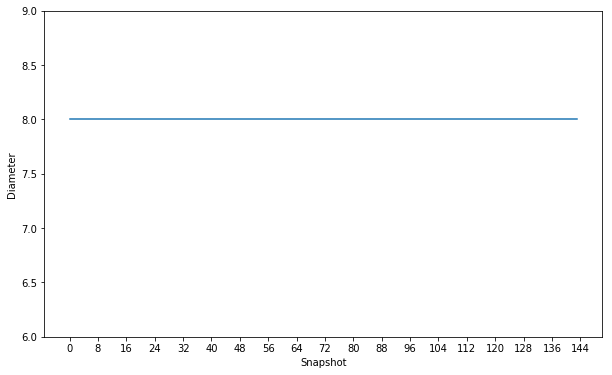
\includegraphics[width=\linewidth]{daily_diameter3}
			\caption{Snapshot, June 2nd}
			\label{daily_diameter3}
		\end{subfigure}
		
		\caption{Diameter trends on a daily basis}
		\label{daily_diameter}
	\end{figure}
	
	The graph diameter is a measures that is derived from the wider notion of \textit{eccentricity} $\epsilon$ which is defined as the greatest shortest distance between a vertex \(v\) and every other vertex and expresses how much a node \(v\) is distant from the farthest node of the graph. The diameter \(d\) is the greatest shortest path among all the pair of nodes, i.e. it is the maximum eccentricity of any vertex in the graph.
	
	\[d = \max_{v \in V} \epsilon(v)\]
	
	The churn rate of the network in all four snapshots is too low to justify a variation, resulting in a constant behavior during each 144 snapshots. These trends were actually showed to justify a wider period of observation as it is hard to infer any properties from the gathered data. In the following sections, the very same trends will be showed with respect to a 32 days period. 

	\subsection{Monthly nodes variation}
	
	\begin{figure}
		\centering
		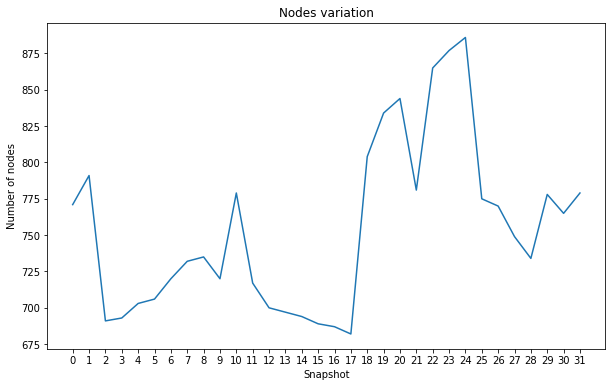
\includegraphics[width=\linewidth]{number_of_nodes}
		\caption{Monthly nodes variation.}
		\label{monthly_nodes}
	\end{figure}
	
	Figure \ref{monthly_nodes} displays the trend of the churning nodes from May 15th to June 27h. Differently from what has been observed on the daily trends, here the overall variation at the end of the observation period is, as expected, more pronounced as the size of the network has seen a +13.73\% joining rate.
	
	\begin{center}
		\begin{tabulary}{\linewidth}{| L | C | C | C | C | C |}
			\hline	
			& Starting nodes & Final nodes  & Variation(\%) & Max num. of nodes & Min num. of nodes \\ \hline
			May 15th - June 27th & 779 & 886 & +13.73\% & 886 & 682 \\ \hline
		\end{tabulary}
	\end{center}
	
	\subsection{Monthly edges variation}
	\begin{figure}
		\centering
		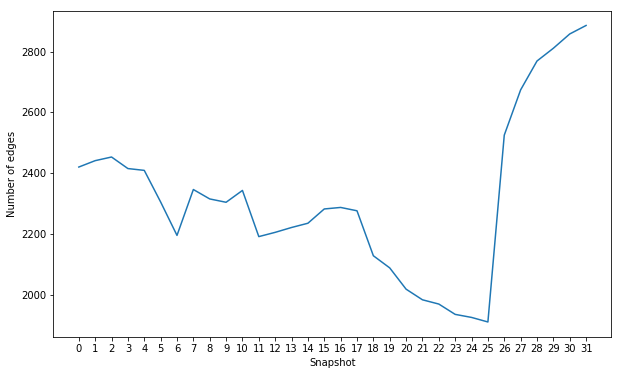
\includegraphics[width=\linewidth]{number_of_edges}
		\caption{Monthly edges variation.}
		\label{monthly_edges}
	\end{figure}

	Edges trend follow the same nodes trend as it has been already showed with the daily trends. Here the gap between highs and lows are even more pronounced due to the fact that it is likely that nodes have more than one channel towards other nodes and this is reflected by the variation observed with respect to the nodes, being it +19.25\%. This graph helps to understand better the dynamic nature of the Lightning Network channels, as the churning rate of edges is higher than the one accounting for the nodes. 
	
	\begin{center}
		\begin{tabulary}{\linewidth}{| L | C | C | C | C | C |}
			\hline	
			& Starting channels & Final channels  & Variation(\%) & Max num. of channels & Min num. of channels \\ \hline
			May 15th - June 27th & 2420 & 2886 & +19.25\% & 2886 & 1910 \\ \hline
		\end{tabulary}
	\end{center}
	
	\subsection{Monthly average degree variation}
	
	\begin{figure}
		\centering
		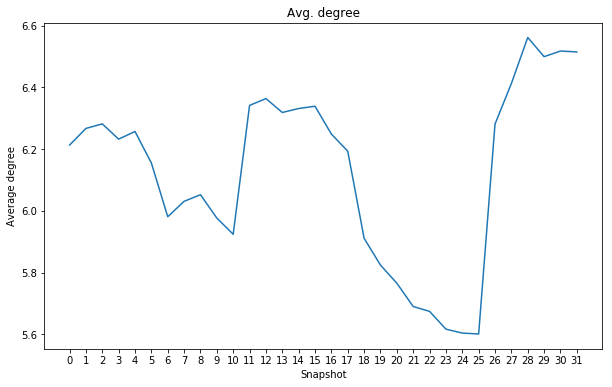
\includegraphics[width=\linewidth]{average_degree}
		\caption{Monthly average degree.}
		\label{monthly_degree}
	\end{figure}
	
	As a consequences for these rates, the average degree of the network oscillates between a higher gap with respect to what has been observed during the daily analysis where the fluctuation was on average +0,67\%. Later it will be showed the actual degree distribution of the graph, and an interesting property that will emerge is that it resembles a power-law distribution. Thanks to this intuition it will be possible to play around this feature in the building of an equivalent model. The following table shows the main characteristics emerged from the overall average degree analysis.
	
	\begin{center}
		\begin{tabulary}{\linewidth}{| L | C | C | C | C | C |}
			\hline	
			& Starting degree (avg.) & Final degree (avg.)  & Variation(\%) & Max avg.degree & Min avg. degree \\ \hline
			May 15th - June 27th & 6.21 & 6.51 & +4.85\% & 6.56 & 5.60 \\ \hline
		\end{tabulary}
	\end{center}
	
	\subsection{Monthly diameter}
	
	The diameter essentially falls within the already known bounds found during their analysis over a daily time window, although, thanks to a wider observation period, it is possible to see how frequent the oscillation between different diameters are. In the case in exam, the plot shows a period in which the network has seen an increase that lasted for 22 days. the importance of this data will be better explained in the next session, but shortly, if a payment uses the geodesic distance as the preferred method to deliver funds, then it would mean that in the worst case there is the need to cross 7 (or 8) channels before reaching the desired peer. Keeping track of this feature may help to balance the network in a way so that new channels can fill the gap between less connected clusters or to be aware of failures of central nodes.
	
	\begin{figure}
		\centering
		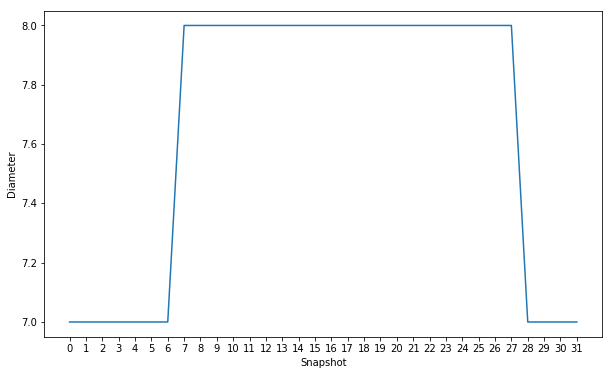
\includegraphics[width=\linewidth]{distance}
		\caption{Diameter.}
		\label{monthly_diameter}
	\end{figure}

	\section{Betwenness	centrality}
	
	The betweenness centrality is a measure of centrality in graph theory based on shortest paths and it was first formalized in 1977 by Freeman, L.\cite{Freeman1977}. The betweenness centrality indicates how much a node in a graph stand between each other shortest paths, and it is a fundamental tool to evaluate the importance of nodes in several fields: for example, in telecommunication systems, a node with a high betweenness centrality means that a large portion of the traffic passes through it, that is, it effectively controls an appreciable part of the network but it also finds applications in biology, social networks, transport networks and many other research fields. 
	
	Since the Lightning Network is a peer-to-peer payment system, it is crucial to understand which are the main players involved as they fulfill the role of bridges of different parts of the network (thus, their disconnection may cause a temporary denial of service) and entry points for new nodes as they offer guarantees over their reliability given the fact that they already manage a high payment traffic (also known as \textit{preferential attachment} property from scale-free network), essentially forming the real backbone of the Lightning Network. But before proceeding with the results of the betweenness centrality measurements it is necessary to talk about the metric chosen to evaluate the shortest path.
	
	The Lightning Network is a payment system based on routes between peers that delegates the payment task to their neighbors thanks to a special contract called HTLC. However, it may happen that a fund that is being processed may end up kept in hostage by a faulty node; therefore, in order to prevent this disruptive scenario a timelock (namely nLockTime parameter) is applied for each HTLC transactions that occur during the payment in order to have the certainty that, after a fixed amount of time, the payment can be considered valid. The best case scenario occurs when all the nodes of a payment path are cooperative and fulfill their duties (i.e. the payment is resolved almost instantly), while the worst case scenario occurs when each node acts maliciously by waiting until the expiration date of the HTLC approaches and then fulfilling their task, as the fidelity bonds between two parties enforce to adhere to the protocol (penalty, the lose of all the liquidity in the channel in favor of the offended party). 
	
	By default, the nLockTime parameter is set to 144 blocks which are approximately 24 hours (the Bitcoin blockchain can be seen as a timestamp service, hence the two expressions are mutual) and we've seen so far that the diameter of the network is around 7 and 8 as showed in Figure \ref{monthly_diameter}. Thus, if the path between two peers has only malicious participant it would mean that a transactions can be considered valid only if 7 days are passed, and the funds gets locked out as well. This is the reason why it is advised to pay only for small amounts of Bitcoins, as larger sums could be locked for several days as they are still considered involved in an open payment operation: if the same situation should happen with larger sums, the consequences would be disruptive for the network as it may prevent peers to fulfill any payment for days; another reason for small payments is that large transfers of money would drain a channel balance instantly, forcing the settlement of the channel after few transactions. A new approach to payments called AMP \cite{Amp2018} - Atomic Multipaths Payment - has been proposed as a workaround to the latter problem. It should be clear to the reader then that a payer has the necessity to minimize the distance between him and his payee, as it will minimize the time required to process a transaction in case of adversarial nodes along the path and also will minimize the time he has to wait before getting his channel funds unlocked and ready to use for a new transaction.
	
	\begin{figure}
		\centering
		\begin{subfigure}{0.45\textwidth}
			\centering
			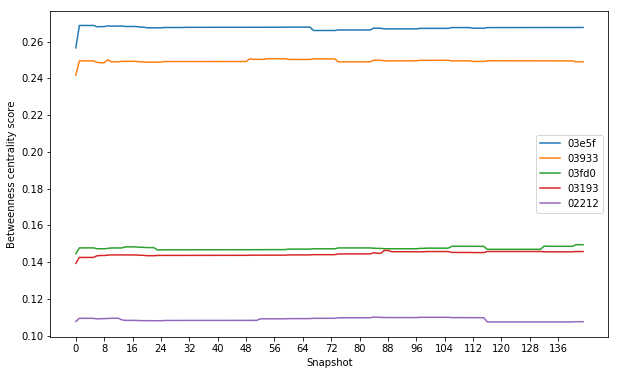
\includegraphics[width=\linewidth]{daily_betweenness_centrality0}
			\caption{Snapshot, May 16th}
			\label{daily_beetwenness0}
		\end{subfigure}
		\begin{subfigure}{0.45\textwidth}
			\centering
			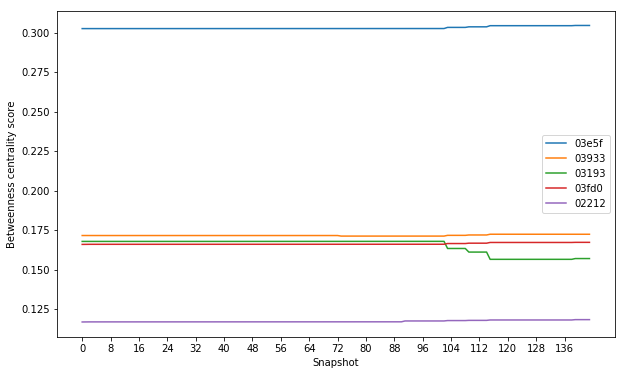
\includegraphics[width=\linewidth]{daily_betweenness_centrality1}
			\caption{Snapshot, May 21th}
			\label{daily_betweenness1}
		\end{subfigure}
		\begin{subfigure}{0.45\textwidth}
			\centering
			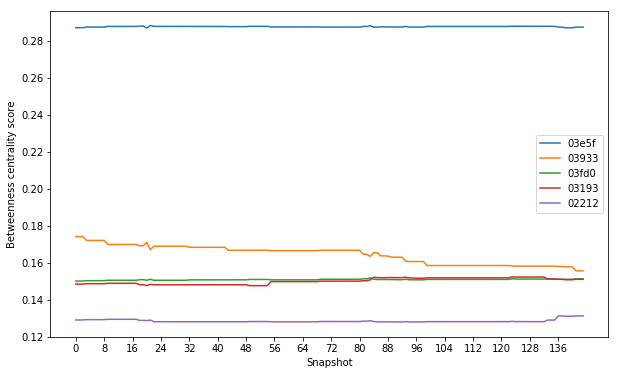
\includegraphics[width=\linewidth]{daily_betweenness_centrality2}
			\caption{Snapshot, May 26th}
			\label{daily_betweenness2}
		\end{subfigure}
		\begin{subfigure}{0.45\textwidth}
			\centering
			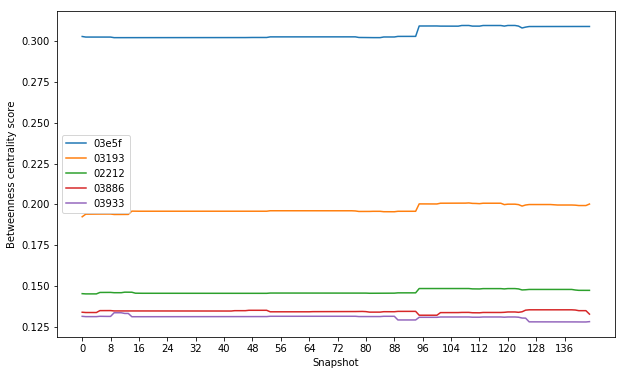
\includegraphics[width=\linewidth]{daily_betweenness_centrality3}
			\caption{Snapshot, June 2nd}
			\label{daily_betweenness3}
		\end{subfigure}
		
		\caption{Betweenness centrality}
		\label{daily_betweenness}
	\end{figure}
	
	It has been observed that more than 90\% of nodes policies carried the default timelock delta value of 144. Since the analysis was carried on the testnet environment it is probable that the policies of the remaining 10\% of the edges were modified for research activities since the Lightning Network authors strongly suggest to stick with the default value for safety reason. After having removed all the edges whose timelock was different from 144, it was safe to assume that the traversal cost of an edge was equal to 1 without loss of generality.
	
	
	As for the algorithm itself that will be used, the Networkx has its own implementation based on the Ulrik Brandes \cite{Brandes2001} variant that computes the betweenness centrality running in $\theta(nm)$ and $\theta(n + m)$ space where $n$ is the number of nodes and $m$ the number of edges whereas the fastest known algorithm at the time required $\theta(n^3)$ time and $\theta(n^2)$ space.	Generally speaking, the betweenness centrality is evaluated according to the formula 
	\begin{equation}
		g(v) = \sum_{s \neq v \neq t}{\frac{\sigma_{st}(v) }{\sigma_st}}
	\end{equation}
	where $\sigma_st$ is the total number of shortest paths from node $s$ and node $t$ and $\sigma_{st}(v)$ is the number of paths that pass through $v$. In order to have $g(v) \in [0, 1]$ it is necessary to normalize the values by dividing (for undirected graphs) by $(N-1)(N-2)/2$ where $N$ is the total number of nodes.
	
	\begin{figure}
		\centering
		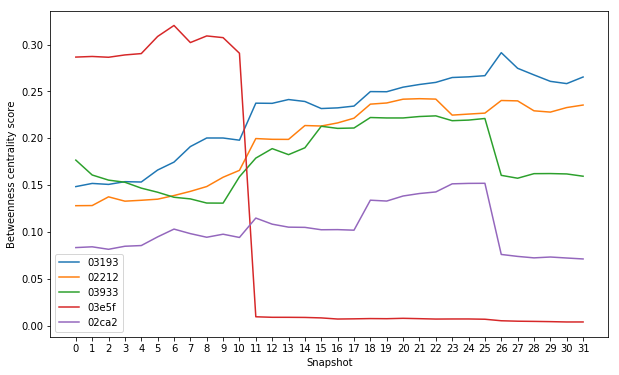
\includegraphics[width=\linewidth]{monthly_betweenness_centrality}
		\caption{Betweenness Centrality (Monthly)}
		\label{monthly_betweenness_centrality}
	\end{figure}		
	
	The data in Figure \ref{daily_betweenness} picks the top 5 nodes according to their betweenness centrality aggregated score. The aggregated score means that the centrality gets first evaluated for every node of the intersection $V = \{V_1 \cap V_2 \cap \cdots V_k \}$, where $k$ is the number of snapshot and $V_i$ being the set of nodes of each snapshot, then
	\begin{equation}\label{eq:betwenness}
		B_i(V) = \{ g_i(v) \mid \forall v \in V \}
	\end{equation}
	is computed, such that $B_i$ is the betweenness centrality score for all the nodes of the $i$-th snapshot. Then the nodes are sorted according to the aggregated score
	\begin{equation}
		B(V) = sort(\{ \sum_{j = 0}^{k}g_j(v) \mid g_j(v) \in B_i(V), \forall i= 0,1,2 \cdots k\})
	\end{equation}
	and the top five elements by score are picked. The reason why this metric has been evaluated over the intersection of nodes is because of the interest in finding the stable backbone of the network.
	
	\begin{figure}
		\centering
		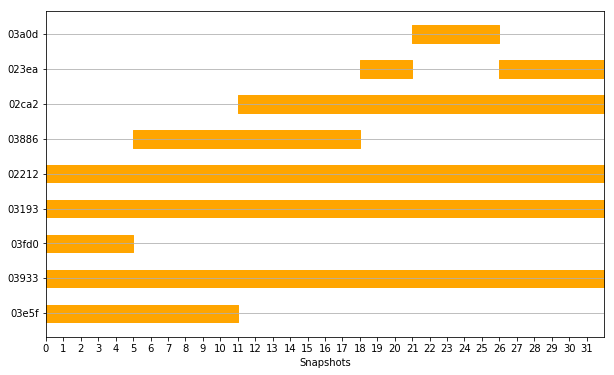
\includegraphics[width=\linewidth]{monthly_gantt_chart}
		\caption{The graph represents the nodes that occupied the first 5 position whose score was the best among the rest of the other nodes.}
		\label{monthly_gantt}
	\end{figure}

	As expected, the scores appear to be constant or with low variations along the 144 snapshots. The nodes are identified by the first five characters of their public key, and by looking at those IDs it emerges that the set is different for all their snapshot meaning that indeed new nodes joined the network during the five days elapsed between each snapshot and attached to already well established nodes. 
	
	This aspect is even more pronounced if we look at Figure \ref{monthly_betweenness_centrality} where the monthly behavior is displayed and thanks to this metric is possible to investigate deeper on nodes and events that occurred during the observation period. 
	
	For example it has been noted that, on average, the total number of neighbors of these five nodes is 486.125, accounting for 62,7\% of the overall size of network. Such a high centrality score also suggests that the neighbors may only have a single channel that keeps them connected to the largest connected component. By removing these five nodes from the latest snapshot, the graph gets partitioned into 234 subgraphs: the largest subgraph among these contains 532 nodes (which is the Lightning Network itself) while the number of nodes of the remaining subgraphs is 242. Of these 242 nodes, 228 were single channel nodes.

	It is then possible to investigate over some peculiar events like the one happened during snapshot 10 and 11, where node \textit{03e5f9} lost suddenly its centrality over 24 hours: 
	from day 0 through day 10 the node was performing first among the others for betweenness centrality score. On day 11, the node dropped from 196 nodes to 37 as it closed channels with 159 peers; out of these 159 peers, 98 of them were single channel nodes, effectively disconnecting them from the rest of the network making node \textit{03e5f9} the single point of failure for the 12\% of the total nodes. Unfortunately it's impossible to determine the causes that led to such a drop as it may be happened because of saturated channel balances, unresponsive nodes or internal errors on their server.
	
	Contrary to Figure \ref{monthly_betweenness_centrality}, Figure \ref{monthly_gantt} shows which nodes occupied the first five positions during the very same period, independently from their aggregated score, that is, the graph shows only the node that were top 5 for each day of the time interval in exam, for a total of 9 nodes that alternates each other throughout the observation period. This plot helps better to understand the stability of a node, since a central node will likely perform better than peripheral nodes when it comes to payments delegation, also we'd like a node that is stable because as it has been showed with node \textit{03e5f9} a crash would be disruptive for the network health.
	
	By looking at the history of the betweenness centrality is then possible to understand better the reliability of particular nodes. It also helps preventing that nodes get too centralized as the network becomes more similar to a centralized hubs network rather than a decentralized one: the autopilot feature of Lightning Network may check the whole network betweenness centrality to balance out the new channels establishment with the current topology in order to decrease the centrality and the maximum diameter of the network. On the other hand, clients may want to give up the decentralization feature to embrace a more reliable 
	
	\newpage
	
	\section{\textit{k}-vertex connectivity}

	\begin{figure}
		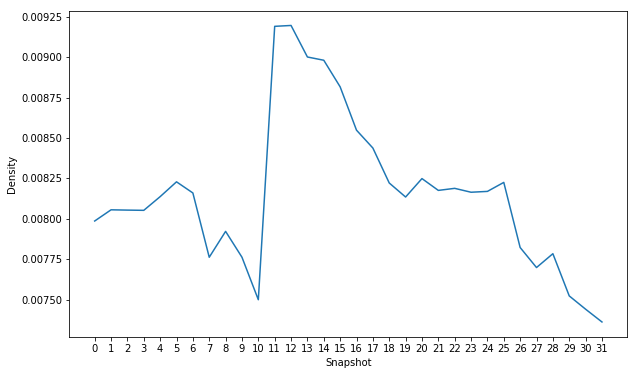
\includegraphics[width=\linewidth]{monthly_completeness}
		\caption{Density of the graphs. Density is calculated as $\frac{m}{n(n-1)}$}
		\label{monthly_completeness}
	\end{figure}
	
	\textit{k}-vertex connectivity gives an important outlook when it comes to robustness. In graph theory a graph $G = (V,E)$ is said to be \textit{k}-vertex connected if for every pair of vertices there are \textit{k}-vertex indipendent paths connecting these vertices, or in other words, \textit{k} is the size of the smallest subset of vertices such that the graph becomes disconnected if deleted. Complete graphs do not fall into this definition since a complete graph cannot be disconnected by removing vertices. Furthemore, if a complete graph has n-vertices, then by the above definition it falls in the class of (n-1)-vertex connectivity, but as Figure \ref{monthly_completeness} shows, the network is far to be complete.

	Computing the k-vertex connectivity alone over the snapshots is not particularly useful as the Lightning Network, being a connected network, will always be a 1-vertex connected graph. Nonetheless, it's very likely that inside the 1-vertex connected component there may be others, stronger, connected components, i.e. there may exists subgraphs whose k-vertex connectivities are higher than their supergraph. This kind of reasoning can be applied iteratively until it's impossible to find any new subgraph whose k-vertex connectivity is higher than their subgraphs.
	
	The algorithm used to perform this task has been proposed by James Moody and Douglas R. White \cite{Moody2003} based on their research over cohesion in social groups. It returns the k-component structure of a graph G, where a k-component is a maximal subgraph of G that has at least node connectivity k. The algorithm works as follow:
	\begin{enumerate}
		\item Compute node connectivity k of the input graph.
		\item Identify all k-cutsets at the current level of connectivity. 
		\item Generate new graph components based on the removal of these cutsets. Nodes in a cutset belong to both sides of the induced cut.
		\item If the graph is neither complete nor trivial, return to 1; else end.
	\end{enumerate}
	
	The algorithm has been running over the 32 snapshots. What emerged is an inherent hierarchical structure of the network where the innermost components shows a high k-vertex connectivity (or cohesive degree) compared to the most peripheral nodes. Trivially, as the connectivity increases, the vulnerability to isolated actions performed unilaterally by some (byzantine) nodes decreases such that the degree of actions of any malicious attacker depends on at least $k$ components of the subgraph.
	
	\begin{figure}
		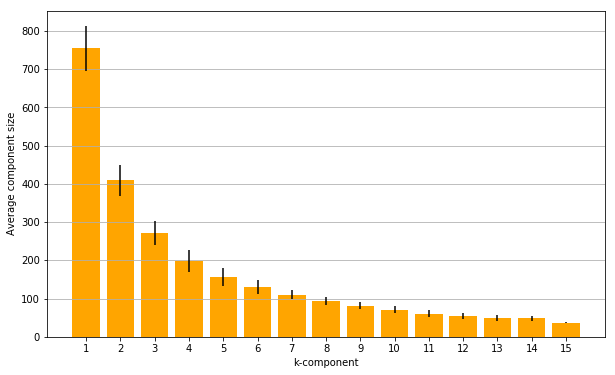
\includegraphics[width=\linewidth]{k_connectivity_average_size}\\
		\caption{Average size for each components for every snapshot taken from May 15th to June 27th}
		\label{monthly_connectivity_average}
	\end{figure}
	
	The data presented in Figure \ref{monthly_connectivity_average} represents the average size of each component over the 32 snapshots in exam. The orange bars represent the mean value of every component while the black lines represent their standard deviation. Even though there are represented up to 15 components, it is not necessary true that the maximum k-vertex size is indeed 15. What the graph suggest is that if there exists a k-component over a particular snapshot, it is likely that the $k$-th component size will be on average like the corresponding value depicted in Figure \ref{monthly_connectivity_average}.
	
	\begin{figure}
		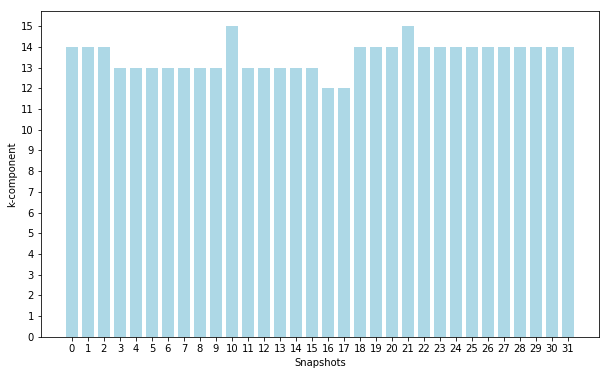
\includegraphics[width=\linewidth]{k_connectivity_max_size}
		\caption{Highest connectivity value for each snapshot.}
		\label{monthly_connectivity_max_size}
	\end{figure}
	
	The 1-connected component is trivially the average of the graph sizes over the 32 captures; indeed every 1-connected component size is equal to the graph order of the relative snapshot. More than 50\% of the network is a biconnected subgraph (2-vertex connected graph) meaning that every node inside it is resilient up to two opportunely selected node failures (that is, nodes selected according to the well-known min-cut criteria) and, as we move right in the plot, the graphs get more and more resistant to node failures. Figure \ref{monthly_connectivity_max_size} depicts the highest value k obtained for each snapshot and shows a dynamic behavior of k-connectivity, ranging from a lower bound of 12 to an upper bound of 15.
	
	It is interesting to see which nodes belong to the top connected component. The intuition is that nodes that scored best in betweenness centrality will likely to belong to the highest k-component. The results were achieved in the following way:
	\begin{enumerate}
		\item Calculate $B_i(V)$ for each snapshot as seen in \ref{eq:betwenness}. Sort the result in a descending fashion. 
		\item For each $B_i(V)$ selects the first $s$ elements, where $s = |C_i|$ and $C_i$ being the set of nodes that belong to highest k-vertex component of the snapshot $i$.
		\item Compute the intersection between the two sets.
	\end{enumerate}
	
	\begin{figure}
		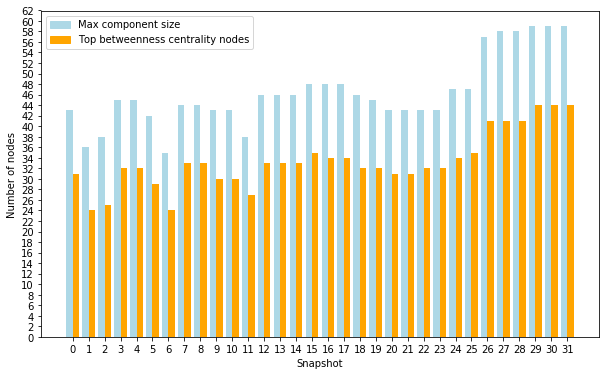
\includegraphics[width=\linewidth]{k_connectivity_beetwenness}
		\caption{text}
		\label{monthyl_k_connectivity_betweenness}
	\end{figure}
	
	The results are showed in Figure \ref{monthyl_k_connectivity_betweenness} and as expect a large portion of the top performing central nodes are inside the innermost connected component.
	
	Dove è stato applicato questo algoritmo
	Cosa ne è uscito fuori (struttura)
	Come è possibile rappresentarne la struttura
	interessanti proprietà (inclusione con la betweenness centrality)
	perchè è interessante analizzarlo
	utilità: sponsorizzare nodi in cui viene promosso il fatto di far parte di una cricca resiliente ai failure
		
	\subsection{Components size}
	\subsection{Betweenness inclusion}
	\section{Max-Cut}
\end{document}